\newcommand{\projectName}{Nail+}


\documentclass{sigchi}

% Use this command to override the default ACM copyright statement
% (e.g. for preprints).  Consult the conference website for the
% camera-ready copyright statement.


%% EXAMPLE BEGIN -- HOW TO OVERRIDE THE DEFAULT COPYRIGHT STRIP -- (July 22, 2013 - Paul Baumann)
% \toappear{Permission to make digital or hard copies of all or part of this work for personal or classroom use is      granted without fee provided that copies are not made or distributed for profit or commercial advantage and that copies bear this notice and the full citation on the first page. Copyrights for components of this work owned by others than ACM must be honored. Abstracting with credit is permitted. To copy otherwise, or republish, to post on servers or to redistribute to lists, requires prior specific permission and/or a fee. Request permissions from permissions@acm.org. \\
% {\emph{CHI'14}}, April 26--May 1, 2014, Toronto, Canada. \\
% Copyright \copyright~2014 ACM ISBN/14/04...\$15.00. \\
% DOI string from ACM form confirmation}
%% EXAMPLE END -- HOW TO OVERRIDE THE DEFAULT COPYRIGHT STRIP -- (July 22, 2013 - Paul Baumann)


% Arabic page numbers for submission.  Remove this line to eliminate
% page numbers for the camera ready copy 

%\pagenumbering{arabic}

% Load basic packages
\usepackage{balance}  % to better equalize the last page
\usepackage{graphics} % for EPS, load graphicx instead 
%\usepackage[T1]{fontenc}
\usepackage{txfonts}
\usepackage{times}    % comment if you want LaTeX's default font
\usepackage[pdftex]{hyperref}
% \usepackage{url}      % llt: nicely formatted URLs
\usepackage{color}
\usepackage{textcomp}
\usepackage{booktabs}
\usepackage{ccicons}
\usepackage{todonotes}
\usepackage{subcaption}
\usepackage{stfloats}

% llt: Define a global style for URLs, rather that the default one
\makeatletter
\def\url@leostyle{%
  \@ifundefined{selectfont}{\def\UrlFont{\sf}}{\def\UrlFont{\small\bf\ttfamily}}}
\makeatother
\urlstyle{leo}

% To make various LaTeX processors do the right thing with page size.
\def\pprw{8.5in}
\def\pprh{11in}
\special{papersize=\pprw,\pprh}
\setlength{\paperwidth}{\pprw}
\setlength{\paperheight}{\pprh}
\setlength{\pdfpagewidth}{\pprw}
\setlength{\pdfpageheight}{\pprh}

% Make sure hyperref comes last of your loaded packages, to give it a
% fighting chance of not being over-written, since its job is to
% redefine many LaTeX commands.
\definecolor{linkColor}{RGB}{6,125,233}
\hypersetup{%
  pdftitle={SIGCHI Conference Proceedings Format},
  pdfauthor={LaTeX},
  pdfkeywords={SIGCHI, proceedings, archival format},
  bookmarksnumbered,
  pdfstartview={FitH},
  colorlinks,
  citecolor=black,
  filecolor=black,
  linkcolor=black,
  urlcolor=linkColor,
  breaklinks=true,
}

% create a shortcut to typeset table headings
% \newcommand\tabhead[1]{\small\textbf{#1}}

% End of preamble. Here it comes the document.
\begin{document}

\title{\projectName{}: Sensing the Strains From Fingernail As Always-Available Input}% on Any Surface

\numberofauthors{3}
\author{%
  \alignauthor{1st Author Name\\
    \affaddr{Affiliation}\\
    \affaddr{City, Country}\\
    \email{e-mail address}}\\
  \alignauthor{2nd Author Name\\
    \affaddr{Affiliation}\\
    \affaddr{City, Country}\\
    \email{e-mail address}}\
  \alignauthor{3rd Author Name\\
    \affaddr{Affiliation}\\
    \affaddr{City, Country}\\
    \email{e-mail address}}\\
}

\maketitle
\begin{abstract}
We present \projectName{}, a nail augmented device that senses user's fingernail contour and bend when force is applied on a surface. Using 3$\times$3 array of 0.2mm strain gauges, \projectName{} is small enough to fit on fingernails, and at the same time, flexible and stretchable.
We evaluate this interface in motion and motionless mode. The system can distinguish swipe gestures with high accuracy (93.2\%). For motionless mode, it can achieve 85.6\% accuracy for classifying different kinds of finger postures.
Since the device is always available, it allows users to perform swipe gestures on surfaces around or touch postures on touch screen devices to enable a variation of application usage.
We also show some example applications such as quick swiping on surfaces around to control smart TV's or touching on touchscreen devices to enable different application short cuts.
% TODO 103 and 104 is pretty much the same.
\end{abstract}

\keywords{Natural User Interface (NUI); Wearable electronics; fingernail; Strain gauges; Machine Learning; Nail pressure;}

\category{H.5.m.}{Information Interfaces and Presentation
  (e.g. HCI)}{Input devices and strategies (e.g., mouse, touchscreen)} 


\section{Introduction}
Recent works have seen new proposals for nail augmented devices in body-attached computing. Fingernails have been widely adopted due to its characteristic of lacking perception. It also has the advantage of being non-obstructive and the most promising place for easy installation and removal\cite{MagNail}. Moreover, nail art have been proposed in previous works\cite{NailDisplay,NailO}. We believe that using nail as a mounting location will become more popular in the future.

% These devices are designed to be non-obstructive, small, lightweight and no disturbing in daily life. 

% In order to increase touch screen mobility, nail is the place which widely adopted for input due to its no proprioception area. Furthermore, it is less disturbing and most promising place due to easy installation and removing\cite{MagNail}. Lastly, nail art is proposed in previous work\cite{NailDisplay,NailO}. 
% In our daily life, we use our fingertips for controlling smart devices and feeling the tactile feedback from surface. Upon on this, flat and smooth touchscreen has been proposed and widely adopted by users. However, touchscreen are not always available device and at most of the device can only have binary states for touching. 
% Fingernail has multiple advantages for body mounted-device.


% 一開始講在nail上面output的work
% 在結尾開始講在nail上面做input的work
Early works on fingernail mounted devices develop schemes to augment fingernails as an output of display and a signal source for sensors.
% TODO 有點怪 please double check
NailDisplay\cite{NailDisplay} mounts a visual display on top of fingernail to avoid the big thumb problem on touchscreen. Ando et al.\cite{NailTDisplay} proposes to put a small voice coil to control the tactile feedback from surface by changing waveforms. More than that, FingerSight\cite{FingerSight} implements a device consisting of a camera to extract environmental information. Previous research also demonstrates using nail-mounted device to enrich input area. NailO\cite{NailO} proposes a capacitive sensor grid on top of the fingernail to sense swipe and tap gestures.
uTrack\cite{uTrack} and FingerPad\cite{FingerPad} places small magnet on the fingertip, and uses a magnetic field to track finger movements. TouchSense\cite{TouchSense} uses 3-axis accelerometer to detect finger postures for switching different modes of input.
These works have proven the advantages of a device mounted on top of fingernails. However, these works have not explored the characteristics of a fingernail itself as a signal source.

\begin{figure}
  \begin{center}
  \includegraphics[width=0.9\columnwidth]{figures/landing.pdf}
  \caption{\projectName\ THIS IS A PLACE HOLDER FOR \projectName{}}
  \label{fig:main}
  \end{center}
  \vspace{-1em}
\end{figure}

% 以下開始討論用指甲本身的特性 像是顏色改變
This brings us to think about using a fingernail as an input property proposed in \cite{NailSense}, which senses force touch via computer vision.
% There are also works using fingernail itself as a sensing part.
Mascaro et al.\cite{Photoplethysmograph} also implements a nail-mounted device for observing changes in the reflection intensity on a fingernail. (one more work!) However, the sensing technique still leaves in question the recognition of swiping gestures and is limited to force sensing which is not enough for daily use.
% TODO 這邊要多加work! 應該要三篇比較ok,大源說要改成還沒explore

In order to explore better sensing technique of nail augmentation, we aim to design a device that achieved the following designs. First, it has the ability of sensing simple gestures (e.g. swiping and tapping) on surfaces. Secondly, it has no restrictions on input area which enable users to perform gestures on surfaces around. Finally, it should come in a light and thin form factor to preserve the unobtrusiveness of fingernails.
The proposed design will be a novel input device for increasing the mobility of touch screen. It also can be perform gestures anywhere without physical effort.

In this paper, we developed a prototype, \projectName{} (\autoref{fig:main}), utilizing a 3$\times$3 array of strain gauges sensor to explore the technique of using strains from fingernail as input.

% mobility  in enhancing the modality of finger interaction, and expanding the interaction space due to the gesture can be performed everywhere.


% 指甲擁有了
% Using body parts as an input sensing technique becomes popular research area in HCI community recently. It not only provides users control surroundings by simply performing intuitively gestures, but also comes as an always-available input device which lowers physical effort when user needed.
% Since the device is mounted to our body, it is important to be attentive for the comfort level which will determines the utility of the device.
% Many form factor of sensing technique are presented (e.g. wristwatches, rings, bends). However, using fingers to perform gesture on surface is already built in our daily life which is widely adopted by users and it is the most intuitive way to perform gestures.



% In this paper, we chose the fingernail as a input area which has no proprioception and the device on top of it can be easily forgotten by user. Furthermore, it is less disturbing and most promising place due to easy installation and removing\cite{MagNail}. Lastly, nail art is proposed in previous work, Kao et al.\cite{NailO} implemented a nail-mounted device to sense swipe gestures on top of fingernail with decorations at top layer.

% Previous research also demonstrated using nail-mounted device to explore new interactions. Hwang et al.\cite{NailSense} proposed a technique which senses the force pressure by detecting white region of fingernail using computer vision. Kadomura et al.\cite{MagNail} also used a magnet on top of finger to enable interaction nearby smart devices with magnet sensor. TouchSense\cite{TouchSense} used 3-axis accelerometer to detect finger postures to switch different modes of input. TapSense\cite{TapSense} use a acoustic way to identify the gestures that drawing on the wall.
% However, the interaction of the techniques are limited to particular sensing area such as the region that can sense touch or within camera site.

% There are also works to track 2d on surface. LightRing\cite{LightRing} used a infrared proximity sensor and gyroscope to track finger movement. FingerPad\cite{FingerPad} and uTrack\cite{uTrack} instrument the fingertip with a small (passive) magnet, and a second finger with an active device that tracks the finger by magnetic field changes. Althought these device are

% To explore better interaction of nail augmented device, we aimed to design a device that have no restrictions of input area which can enable user to perform gestures on surfaces around. 
% The proposed technique will definitely be helpful in enhancing the modality of finger interaction, and expanding the interaction space due to the gesture can be performed everywhere.(this should be changed as well because this is a copy from nailsense) Our prototype, \projectName{} (\autoref{fig:FIGURE1}), use a 3$\times$3 array of strain gauges sensor. The size of the device's height is 0.8cm and width is 1cm which is smaller than 1 cent of US dollar.
% Derived from NailO\cite{NailO}, we aimed to provide a technique that can sense a touch and swipe event on any surface around user, and explore a touch using strain features to distinguish different kinds of posture and swipe gestures. We implemented a nail-mounted device that can sense the slight strain changes from fingernail when finger touches the surface. By letting user perform gesture on surface, user can perform gesture more intuitively. 
% 
% To better explore the ability of the strain from fingernail, we aimed to 
% Wolf et al.\cite{LightRing} provides a ring that can track 
% Products such as nail art stickers and fake eyelashes are widely accepted as extensions to the body for decoration and self-expression. They seamlessly blend into our physical bodies when attached, and are easily removable. As people already wear these products for fashion purposes, we propose embedding technology into these products to extend their functionality and utility to interaction.bodies when attached, and are easily removable.
% 
% Products such as nail art stickers and fake eyelashes are widely accepted as extensions to the body for decoration and self-expression. They seamlessly blend into our physical bodies when attached, and are easily removable. As people already wear these products for fashion purposes, we propose embedding technology into these products to extend their functionality and utility to interaction.
% To afford usability in the form of cosmetic extensions, three main design themes must be realized: First, the interface should be small and unobtrusive. It should be designed with technology that can be miniaturized to the size of cosmetic products. When worn, it should be comfortable to an extent its existence could be forgotten. Second, the interface should afford natural interactions. The interactions should be simple, intuitive and require minimal cognitive mapping, building on natural body gestures. Third, the interface should be appealing and easy to wear. Like clothing and accessories, the interface can be easily customized. The mounting and removal process should also be simple and similar to existing cosmetic processes. As no device exists that satisfies the above criteria, our work is motivated to do so.



%must have this!
In summary, the main contributions of this paper are as follows:
 \begin{itemize} %placeholder for now
 \item A novel fingernail input interface presented and explores the ability of fingernail's strains as a input technique.
 \item We develop a nail-mounted prototype can detect swipe gestures and postures of fingernail.
 \item We conducted two system evaluations of this technique and implemented scenarios to explore interactions.
 \end{itemize}



% \section{Related Work}
% \subsection{Functional work}
% LightRing\cite{LightRing} provides an always-available 2D input on any surface. LightRing uses IR emmitter and gyroscope to acquire finger movements on any surface. IR emmitter is used for measuring the distance between the ring and the middle segment (middle phalanx) of the instrumented finger, and gyroscope is used for rotation rate. However, it need to correct for drift with a magnetometer for other longer interactions.
% \subsection{Camera Approches}
% NailSense\cite{NailSense} use camera to track the finger tip’s color change, and then guess user is performing the touch or released gestures (using OpenCV). The limitation is camera needed and the gestures need to be performed in front of it. AirPincher is a handheld device which provides eye-free input within fingers and support 6 kinds of gesture with tactile feedback. User can use his/her thumb to pinch, swipe, rubbing at index and middle finger, and the demo of surfing websites also proposed. Nevertheless, camera needed and need to hold the device, not always available.
% \subsection{Location work}
% MagNail\cite{MagNail} is a study that augmenting nails with a magnet to detect user actions using a smart device which allows user actions to be detected via the magnetic sensor integrated in smart devices such as a smartphone or a tablet PC. The limitation is the error rates is pretty high on the button of the device. NailO use capacitive sensing on printed electrodes as a input surface. It is small and unobtrusive, existence could be forgotten and it has a high accuracy. However, it can only support 5 kinds of gestures. 
% \subsection{Acoustic work}
% TapSense\cite{TapSense} use a acoustic way to identify which gesture is preformed by the users. They capture the sound when our fingers strike the screen, and use that sound pattern to recognize the gesture. This approach doesn't require user to wear anything, but will need a microphone which already built in smart phones. Scratch input use the sound when fingernail is dragged over the surface of a textured material as finger input surface. Six Scratch Input gestures at about 90\% accuracy with less than five minutes of training and on wide variety of surfaces. However, the interface table will not always exist.

\section{Prototype Design}
To design a nail augmented device for touch or gesture sensing, few main requirements were met. First of all, the device must be small enough to fit within fingernail. Second, it should have ability of sensing slightly changes of the strain from fingernail. Last but not least, it has to be reusable and easy for installation and removing. Based on above of requirements, we derived that using a 2D array of 0.2mm strain gauges is the appropriate solution for this prototype. To derive a general fitting, we conducted a pilot study to collect the average size of fingernail.

\subsection{Pilot Study : Size of Fingernail and Human Behaviour}
We recruited 10 participants (7 male, 3 female) from ages 20 and 24 (mean 21) to find an average width and height of fingernail. We also requested users to perform tap gesture on electronic load-cell to measure how much pressure is normally applied on a surface to investigate the ability of strain gauges.
The result of this pilot study, fingernail width is 1.145cm (SD=0.14) and height is 1.21cm (SD=0.17). 
And the average of tap pressure measured 0.82N (SD=0.26).
% The changes of color on fingernail are obvious when we press pressure changes, 

% , trains from fingernail is 

% Physical changes on the surface of nail caused by finger motions and gestures on surface are visible to the human eye. However, there is still difficulty on detecting it through most sensing techniques because such physical changes are very small in comparison to that of finger joint movements. Moreover, physical changes on the surface of nail varies from person to person. Accordingly, we have two major requirements. First, a small and light device must be able to sense small physical changes. Second, a device must be able to extract individual information from multiple spots on the surface of a human nail. Among a variety of sensing techniques, we conclude that strain gauge sensors best fit our requirements for this prototype.

% \begin{figure}[t]
%   \includegraphics[width=1\columnwidth]{figures/CompleteDiagram_v3.pdf}
%   \caption{The complete circuit diagram. Note that SG stands for strain gauge. The 16:1 analog multiplexer is practically made up of 3 analog multiplexers.}
%   \label{fig:completeCircuitDiagram2}
% \end{figure}

% TODO pilot前綴?
% TODO 3x3 array issue.
\subsection{Hardware}
% The device is height 0.8cm and width 1.0cm
We developed \projectName{} using a 3$\times$3 array of 120-ohm 0.2-mm strain gauges for sensing part (Shown in \autoref{fig:main}). Below the strain gauges, we used a stretchable and flexible artificial-skin to adhere sensors onto user's fingernail. The size of it only takes 0.9cm$\times$1cm which is smaller than 1 US cent, and the thickness of it is 1mm. Each of the strain gauge is directly wired to the computing part.
The computing hardware is consisted of an Arduino Nano board and two 8-to-1 analog switches(MAX4617, Maxim Integrated), a dual digital potentiometer (AD5231, Analog Devices), and two instrumental amplifiers (AD623 and INA122U, Analog Devices). 
% TODO check hardware
% hardware confirmed!!


The diagram of the computing hardware is shown in \autoref{fig:completeCircuitDiagram}. First, the multiplexers are sequentially selected to connect one of the strain gauges. Upon one of the strain sensors is selected, it becomes one of the four resistors on the Wheatstone bridge. When the forces apply on fingertip, the strain of fingernail let the sensor slight bend or contour which causes the ohm value of strain gauges lower or higher. Due to the changes of ohm value, one side of the voltage in Wheatstone bridge also changed. This difference becomes our sensing signal input.

\begin{figure}[t!]
  \hspace{-2em}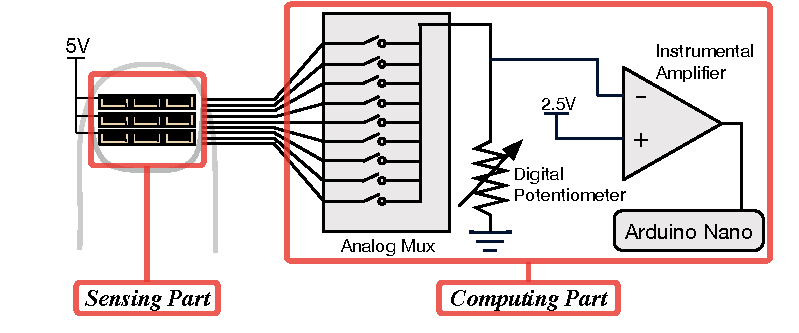
\includegraphics[width=1.1\columnwidth, height=0.47\linewidth]{figures/CompleteDiagram_v4.pdf}
  \caption{The complete circuit diagram. Sensing part is consisted with 9 strain gauges. For computing part, we actually used two analog multiplexers and the instrumental amplifier is made up of two amplifiers as well.}
  \label{fig:completeCircuitDiagram}
  \vspace{-0.8em}
\end{figure}

Due to the requirement of sensing the slightly change of the strain from fingernail, we used two amplifiers to magnify the difference on the two sides of Wheatstone bridge 4000 times. Finally, Arduino Nano reads the final analog value from the last amplifier's output. For the digital potentiometer, it is used for adjusting the resistance to let the Wheatstone bridge have no difference on both side during calibration.


\subsection{Gesture / Posture Recognition}
We used LIBSVM tool\cite{libsvm}, a popular machine learning open-source library for SVM which is a way to distinguish the pattern by vectors.
Since the different type of the input data sets, we implemented two algorithm specifically for swipe gestures (Motion mode) and finger posture (Motionless mode).
In motion mode, sequentially and time based data is preprocessed by accumulating each data's difference from the first received data when the gesture began. At the end, the sequentially data is processed to be one feature data.
In motionless mode, raw data is directly used for machine learning.
For each mode, we scale data's feature to the range of -1 to 1 and then train a multi-class SVM classifier with a Radial Basis Function (RBF) kernel.
%\begin{figure*}[bp]
% \begin{center}
%  \setcounter{figure}{5}
%  \hspace{-1em}\includegraphics[width=2\columnwidth]{figures/mixedconfusingMatrix.pdf}
%  \caption{
%    Motionless mode: Confusing Matrix for each pressure level. Note that \textit{N} stands for Newton, \textit{P} stands for pitch and \textit{R} stands for roll.
%  }
%  \vspace{-1em}\label{fig:postureMatrix}
%  \end{center}
%\end{figure*}
\section{System Evaluation}
The goal of the study is to explore: (1) The system is capable for classifying different kinds of swipe gestures when user perform gesture on surface. (2) Finger posture angles can be identified at user daily usage pressure level. (3) The device is able to sense a force touch. 

\subsection{Participants}
We recruited 10 participants (7 male, 3 female) between the ages of 20 and 23(mean 21.3). All participants are right-handed and drew with their right index fingers on the surface. Each participants received \$5 after one hour experiment.
\subsection{Apparatus} %設備!
We used the load-cell (Error: $\pm 0.5$ grams) which is the same in our previous pilot study. In this experiment, we instrumented a 9 degree of freedom (9DOF) sensor on user's index finger. Since the strain gauges are very sensitive to the strain, we avoid 9DOF sensor to contact fingernail. And the 9DOF sensor is only used for checking whether user is performing the applicable position and angle for collecting data. The surface we used in our study is medium-density fibreboard.

\begin{figure}[t!]
	\begin{center}
  \includegraphics[width=0.9\columnwidth]{figures/apparatus.pdf}
  \end{center}
  \caption{The apparatus in our user study. At the surface, we put a load-cell sensor below (b). For each user, we put a 9DOF (c) sensor on finger and our \projectName{} device on fingernail.}
  \label{fig:apparatus}
\end{figure}

\subsection{Task and Procedure}

\subsubsection{Motion Mode}
We chose four swipe direction (up, down, left, right) and tap for this study.
% as shown in \autoref{fig:swipegestures}.
Users were requested to perform gestures shown on computer screen in front and press space key on keyboard at the beginning and at the end of the gesture. On the desk, we draw instructions of swiping to insure swipe direction and distance is the same for users. Each direction are randomly selected to show on screen, and collected with 10 sets of sequentially data which has total 80 trials for each user. Before the study, a calibration is needed for the first time wearing, and no calibration within this study.

\subsubsection{Motionless Mode}
In this mode, we tried to varies of finger postures with different pressure levels.
For each trail, the participants were instructed to adjust their finger pitch and roll angle which are partially selected from \cite{UnderstandingTouch}. We only chose the angles which are easy to identify by users, and gesture set is shown in \autoref{fig:fingerposture}.
The forces are chosen from our pilot user study, following as average force (0.8N), one SD forces (0.6N, 1.0N), two SD forces (0.4N, 1.2N). The participants were asked to straighten finger during all experiment. In front of the user, there is also a screen showing current (sensing from 9DOF and load-cell sensor) and instructed angle and force. Before each trail, participants were requested to return the initial position. When participants adjust finger to the correct posture and perform correct pressure (tolerance: $\pm 5$grams) on the surface, we start to collect data. Once posture or pressure is inapplicable during the study, recorder will automatically skip the data. For each user, we collect 5 postures with 5 forces for 5 times, which is total 125 trials.
\begin{figure}[t!]
\setcounter{figure}{3}
  \includegraphics[width=1\columnwidth]{figures/fingerposture.png}
  \caption{Motionless posture sets: (a) pitch 15 degree, (b) pitch 45 degree, (c) pitch 15 degree and roll 45 degree, (d) pitch 45 degree and roll 45 degree}
  \label{fig:fingerposture}
  	\vspace*{-2ex}
\end{figure}


\subsection{Results}
%\textit{Accuracy:} is defined as the number of correctly classified samples divided by the total number of samples.



\subsubsection{Motion Mode}
The result of this study is shown in \autoref{fig:swiperesult}. Off-line accuracy was computed using 10-fold cross-validation of the evaluation data. The mean accuracy across all participants is 93.2\%(SD: $\pm 5.98$\%). Most of the error occurred in swiping down and up, likely because the higher friction caused user performed gestures lightly from surface which caused strain on fingernail does not observable for sensor.

\begin{figure}[b!]
	\begin{subfigure}{0.2\textwidth}
	\hspace{-0.5em}\includegraphics[width=1.0\linewidth, height=1.0\linewidth]{figures/swipeconfusing.pdf} 
%	\caption{Caption1}
%	\label{fig:subim1}
	\end{subfigure}
	\begin{subfigure}{0.26\textwidth}
	\vspace*{1ex}\includegraphics[width=1.0\linewidth, height=0.8\linewidth]{figures/swipeAcc.pdf}

%	\caption{Caption 2}
%	\label{fig:subim2}
	\end{subfigure}
	 
%	\caption{Caption for this figure with two images}
%	\label{fig:image2}


%  \includegraphics[width=1\columnwidth]{figures/swipeconfusing.pdf}
  \caption{Motion mode: Confusing Matrix and Accuracy for four direction swiping and tapping. }
  \label{fig:swiperesult}
  \vspace*{-2ex}
\end{figure}

% 此部分數據已確認!!
%\begin{figure}[t!]
%  \includegraphics[width=1\columnwidth]{figures/fingerposture.png}
%  \caption{Swipe Gestures in user study}
%  \label{fig:swipegestures}
%\end{figure}


% 這邊可以說符合一般人的按壓程度

\begin{figure}[hb!]
	\begin{subfigure}{0.2\textwidth}
	\hspace{-0.62em}\includegraphics[width=1.01\linewidth, height=1.0\linewidth]{figures/overallConfusingMatrix.pdf} 
%	\caption{Caption1}
%	\label{fig:subim1}
	\end{subfigure}
	\begin{subfigure}{0.26\textwidth}
	\vspace*{1ex}\includegraphics[width=1.0\linewidth, height=0.7\linewidth]{figures/postureAcc.pdf}

%	\caption{Caption 2}
%	\label{fig:subim2}
	\end{subfigure}
	 
%	\caption{Caption for this figure with two images}
%	\label{fig:image2}


%  \includegraphics[width=1\columnwidth]{figures/swipeconfusing.pdf}
  \caption{Motionless mode: Mixed-force confusing Matrix and Accuracy for each level of pressure.}
  \label{fig:postureResult}
  \vspace*{-2ex}
\end{figure}

\subsubsection{Motionless Mode}
% TODO 這邊要改
% In each trial, after the participant indicated his readiness, one of the drawings in Figure 3 appeared on a Keynote slide. The participant was asked an eyes-free input, that is, not to look at his left palm when sketching on it by right index finger; also, the starting point and stroke order of each drawing were provided. The trial was completed when the participant finished the sketch and dropped his right arm to get ready for the next trial.%During the trial, the participant needed to wear a partial blind- fold modified from a sanitary mask to completely occlude the users view of his hand as shown in Figure 2.
The accuracy due to chance was 20\%. Off-line accuracy was computed using 5-fold cross-validation of the evaluation data. The mean accuracy for mixed all force data together across all participants was 76.9\% (SD: $\pm$13.17\%). The confusing matrix for each force level is shown in \autoref{fig:postureResult}, which shows that the higher pressure level the better accuracy gets. So if we drop 0.4N and 0.6N data, the accuracy can reach 82.44\% (SD: $\pm$12.74\%). Note that most of the error happened in the angle of pitch 45 degree with roll 45 degree. We think it is due to the user sometimes perform postures directly using fingernail instead of fingertip to touch the surface when the roll angle is higher. This caused strain gauges different value for each trail which raise this error classification. For sensing force touch, we used 5-fold cross-validation to evaluate. However, it shows that it can only distinguish 0.4N and 1.2N pressure with 70\% (SD: $\pm$12.74\%) accuracy.
% TODO 此部分數據尚未確認!!

%and the caused of the this due to the user sometimes perform postures directly using nail to touch the surface which caused strain gauges different value. We also run 10-fold cross-validation for our pressure value. It turns out that the device cannot distinguish the difference of slightly changes of pressure. The device only can distinguish the pressure level of difference with 90\% accuracy when it comes to 0.4N with 1.2N.



\section{Example Application}
Based on the advantage of \projectName{}, we show two examples using this new interaction technique and are included in video.
\subsection{Controlling Smart TV / Devices}
In scenario of using smart TV, we always need to take out the remote for controlling. With \projectName{}, user can focus on the TV program without disturbing and physical effort for taking out remote. User can use couch as input surface to perform simply tap and swipe gestures for switching channels and selecting. More than this, we also implement this on smart watch. Due to small screen of the watch, it is very handy that using swipe gesture on surface as reply message or declining phone call.

\subsection{Short cuts within application}
For touchscreen, most of the devices only can distinguish binary state of touch. Using \projectName{}, user can use different finger posture for enable short cuts like right click on computer. For instance for the file system on smart phone, user can use 45 degree of roll angle to show up a short cut drop-down list to delete, move, and change the file name.


\section{Limitation and Future Work}
\textit{Firmly sticker on fingernail:} In our evaluation of system, we noticed that the artificial-skin became not sticky enough through time passing and many times of usage. This caused the misclassifications in this situation due to sensing part separate from fingernail.

\textit{Minimise computing part and Power consumption:} As shown in \autoref{fig:main}, we currently put the computing part at wrist as a wristband form factor. The form factor is limited to Arduino Nano board size. This motives us to minimise the computing part such as a ring form factor in future work. For the power consumption, we currently use 120-ohm strain gauges which can be replaced by much higher ohm like 500-ohm.

\textit{Sensing from all fingers:} Mounting the device all over our fingernail is also our future work. Since more finger evolved in this input technique, we can easily enable more functionality such as multi-touch input like pinch and zoom. 

%黏不緊的問題
% 做到像是筆tracking的部分,偵測角度加上移動方向

\section{Conclusion}
In this paper, we evaluated using strains from fingernail as a input technique. We developed a nail-mounted device called \projectName{}, which is light and small enough to fit on top of fingernails. Evaluation of the this shows that it can distinguish swipe gestures on surface in high accuracy (93.2\%). Not only for swiping but also the finger postures can identify five different kinds of finger posture at average force level with 82.22\% accuracy. The system is also attractive for a nail-mounted always-available input for surface around which enrich the mobility of touchscreen. We also implemented applications for this technique, including remote controlling smart TV and watches and enabling short cuts on touchscreen device. Our currently plans are to extend this system to all fingers input.

% \subsection{Title and Authors}
% \subsubsection{Sub-subsections}
% $\times$
% \texttt{.cls}

%%%

% Use a numbered list of references at the end of the article, ordered
% alphabetically by first author, and referenced by numbers in
% brackets~\cite{ethics, Klemmer:2002:WSC:503376.503378,
%   Mather:2000:MUT, Zellweger:2001:FAO:504216.504224}. For papers from
% conference proceedings, include the title of the paper and an
% abbreviated name of the conference (e.g., for Interact 2003
% proceedings, use \textit{Proc. Interact 2003}). Do not include the
% location of the conference or the exact date; do include the page
% numbers if available. See the examples of citations at the end of this
% document. Within this template file, use the \texttt{References} style
% for the text of your citation.

% Your references should be published materials accessible to the
% public.  Internal technical reports may be cited only if they are
% easily accessible (i.e., you provide the address for obtaining the
% report within your citation) and may be obtained by any reader for a
% nominal fee.  Proprietary information may not be cited. Private
% communications should be acknowledged in the main text, not referenced
% (e.g., ``[Robertson, personal communication]'').
%
%\begin{table}
%  \centering
%  \begin{tabular}{r c c}
%    \toprule
%    & \multicolumn{2}{c}{\small{\textbf{Caption}}} \\
%    \cmidrule(r){2-3}
%    {\small\textbf{Objects}}
%    & {\small \textit{Pre-2002}}
%    & {\small \textit{Current}} \\
%    \midrule
%    Tables & Above & Below \\
%    Figures & Below & Below \\
%    \bottomrule
%  \end{tabular}
%  \caption{Table captions should be placed below the table. We
%    recommend table lines be 1 point, 25\% black. Minimize use of
%    unnecessary table lines.}~\label{tab:table1}
%\end{table}

%\begin{figure*}
%  \centering
%  \includegraphics[width=2\columnwidth]{figures/map}
%  \caption{In this image, the map maximizes use of space. You can make
%    figures as wide as you need, up to a maximum of the full width of
%    both columns. Note that \LaTeX\ tends to render large figures on a
%    dedicated page. Image: \ccbynd~ayman on
%    Flickr.}~\label{fig:figure2}
%\end{figure*}

% \begin{itemize}
% \item text
% \end{itemize}
% \ref{tab:table1}

% \begin{enumerate}
% \item text
% \end{enumerate}


%\section{Acknowledgments}
%
%Sample text: We thank all the volunteers, and all publications support
%and staff, who wrote and provided helpful comments on previous
%versions of this document. Authors 1, 2, and 3 gratefully acknowledge
%the grant from NSF (\#1234--2012--ABC). \textit{This whole paragraph is
%  just an example.}

% Balancing columns in a ref list is a bit of a pain because you
% either use a hack like flushend or balance, or manually insert
% a column break.  http://www.tex.ac.uk/cgi-bin/texfaq2html?label=balance
% multicols doesn't work because we're already in two-column mode,
% and flushend isn't awesome, so I choose balance.  See this
% for more info: http://cs.brown.edu/system/software/latex/doc/balance.pdf
%
% Note that in a perfect world balance wants to be in the first
% column of the last page.
%
% If balance doesn't work for you, you can remove that and
% hard-code a column break into the bbl file right before you
% submit:
%
% http://stackoverflow.com/questions/2149854/how-to-manually-equalize-columns-
% in-an-ieee-paper-if-using-bibtex
%
% Or, just remove \balance and give up on balancing the last page.
%
\balance{}


% REFERENCES FORMAT
% References must be the same font size as other body text.
\bibliographystyle{SIGCHI-Reference-Format}
\bibliography{sample}

\end{document}

%%% Local Variables:
%%% mode: latex
%%% TeX-master: t
%%% End: